\documentclass[10pt,twocolumn,letterpaper]{article}

\usepackage{cvpr}
\usepackage{times}
\usepackage{epsfig}
\usepackage{graphicx}
\usepackage{amsmath}
\usepackage{amssymb}

% Include other packages here, before hyperref.

% If you comment hyperref and then uncomment it, you should delete
% egpaper.aux before re-running latex.  (Or just hit 'q' on the first latex
% run, let it finish, and you should be clear).
\usepackage[breaklinks=true,bookmarks=false]{hyperref}

\cvprfinalcopy % *** Uncomment this line for the final submission

\def\cvprPaperID{****} % *** Enter the CVPR Paper ID here
\def\httilde{\mbox{\tt\raisebox{-.5ex}{\symbol{126}}}}

% Pages are numbered in submission mode, and unnumbered in camera-ready
%\ifcvprfinal\pagestyle{empty}\fi
\setcounter{page}{4321}
\begin{document}

%%%%%%%%% TITLE
\title{Artistic Style Transfer - Midterm Report}

\author{Suyan Qu\\
University of Wisconsin - Madison\\
Madison, WI 53706\\
{\tt\small squ27@wisc.edu}
}

\maketitle
%\thispagestyle{empty}

%%%%%%%%% ABSTRACT
\begin{abstract}
   Artistic style transfer is to apply the style of one image, the style image, typically a painting with special texture, to another image, the content image. The generated image will preserve the content presented in the content image while having the same style and texture of the style image. This project will explore the use of convolutional neural networks in the task of artistic style transfer. 
\end{abstract}

%%%%%%%%% BODY TEXT
\section{Current Progress}
Currently, a simple model proposed by Gatys et al~\cite{Gatys} has been built. It takes in two images, a style image, and a content image, and generates an output image of contents in the content image, but in the same style as the style image. Below are some sample outputs. \\
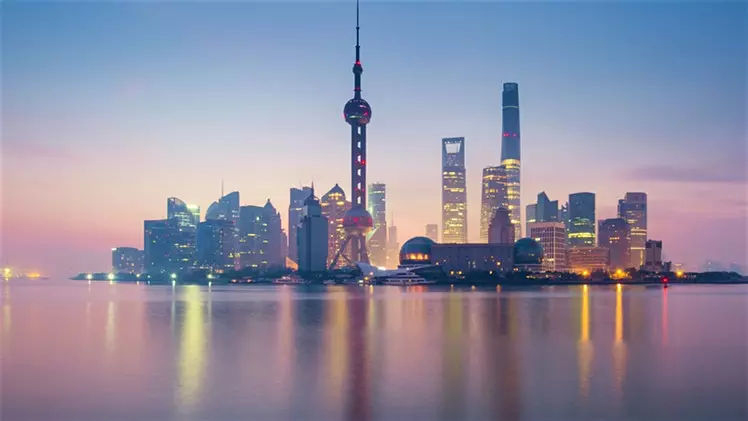
\includegraphics[width = 240px]{city1.jpg} 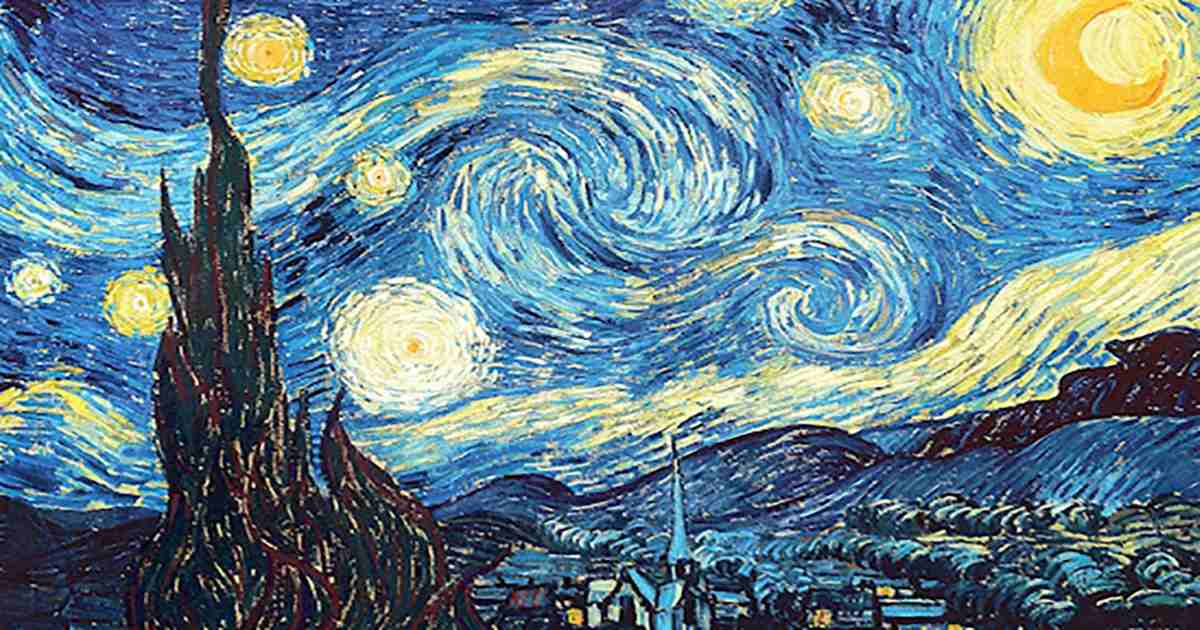
\includegraphics[width = 240px]{starry_night.jpg} 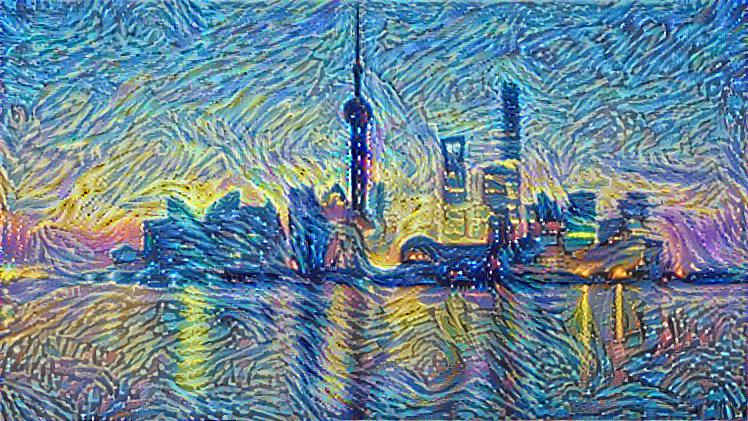
\includegraphics[width = 240px]{shanghai_styled.jpg}\\

%------------------------------------------------------------------------
\section{Difficulties}
In a deep learning neural network. generally the shallow layers can extract some more basic, foundamental features of the input, while the deeper layers can extract some more abstractive features. This model, developped according to this idea, defines style loss as the difference between the output of deeper hidden layers when the content image and the style image are passed into the pre-trained VGG model, then this loss is used to modify the content image. Yet to do this, both the style image and the content image need to be able to fit in the VGG model. In order to generate an image of the same size as the input, a model with the same structure as the VGG model except the input size is created and the weights of the VGG model are loaded to this model. The input size is determined when the content image is loaded into this model. However, the style image may still not be able to fit in this model. The current solution is to resize the style image, but resizing will lead to loss in image quality and distortion, which are not desirable. A better solution is to extract the style~\cite{Ulyanov}, which will be explored in next step. \\
Another major disadvantage of this model is that this model is slow to run. It may take over half an hour to generate an image of $1200\times 800$. Therefore, another direction to improve this model is to accelerate this process and produce real-time style transfer~\cite{Johnson} ~\cite{Ulyanov2}

%-------------------------------------------------------------------------
\section{Update Plan}
The current progress of this project matches the expectation in the proposal, so no change will be made. 

{\small
\bibliographystyle{ieee_fullname}
\bibliography{egbib}
}

\end{document}
